% =====================================================================
%  Relatório Parcial (entrega parcial / midterm) — TCC
%  Sistema Inteligente de Monitoramento Postural
%
%  Parte 1 (Introdução + Revisão Bibliográfica): reproduz a versão já
%  entregue (INTRODUCAO_TCC.pdf). Partes 3–6 (Metodologia, Resultados
%  Parciais, Limitações, Próximas etapas): progresso desta parcial.
%
%  Compilar:  pdflatex relatorio_parcial.tex   (rodar 2x p/ referências)
%  As figuras vêm de ../analysis/figures/ (geradas pelos scripts em
%  analysis/; regenerar com os comandos citados em cada legenda).
% =====================================================================
\documentclass[12pt,a4paper]{article}

\usepackage[utf8]{inputenc}
\usepackage[T1]{fontenc}
\usepackage[brazil]{babel}
\usepackage{lmodern}
\usepackage[margin=2.5cm]{geometry}
\usepackage{graphicx}
\usepackage{booktabs}
\usepackage{amsmath}
\usepackage{textcomp}
\usepackage{gensymb}      % \degree e \ohm em modo texto/mat
\usepackage{float}
\usepackage{enumitem}
\usepackage[hidelinks]{hyperref}
\usepackage{caption}

% figures resolve both in a flat Overleaf project (report/figures/) and in the
% repo layout (../analysis/figures/, where the analysis scripts write them).
\graphicspath{{figures/}{../analysis/figures/}}
\setlength{\parskip}{0.6em}
\setlength{\parindent}{0pt}

% --- Legendas no padrão ABNT: "Figura N – Título" / "Tabela N – Título" ---
\captionsetup{labelsep=endash}
% Linha de "Fonte" (fonte menor), colocada ABAIXO da figura/tabela.
\newcommand{\fonte}[1]{\par\vspace{2pt}{\footnotesize Fonte: #1}}

\title{\textbf{Sistema Inteligente de Monitoramento Postural}\\[0.3em]
\large Relatório Parcial}
\author{André Thomas Monteiro}
\date{Junho de 2026}

\begin{document}
\maketitle

\begin{abstract}
\noindent
Este relatório parcial apresenta o progresso de um sistema inteligente de
monitoramento postural composto por uma cadeira instrumentada com sensores de
pressão (FSR402) e uma unidade vestível com IMU (XIAO nRF52840 Sense) usada na
parte superior das costas. Nesta etapa \textbf{não se monta o sistema integrado}:
cada canal de sensoriamento é caracterizado \textbf{isoladamente em bancada}, com
o hardware já disponível, produzindo as primeiras evidências de viabilidade. No
canal IMU, a remontagem do sensor desloca a referência de ``ereto'' em
$\sim$8{,}0\degree{} (pitch) e $\sim$21{,}6\degree{} (roll), justificando a
calibração por usuário (OE1); o sensor separa 5 de 6 posturas, falhando apenas no
par curvar-para-frente {\itshape vs.} cabeça-baixa (distância de centroides
6{,}9\degree{} contra $\geq$21{,}7\degree{} nos demais pares) --- o que motiva
diretamente a fusão com os FSR. No canal FSR, a resposta satura e deve ser tratada
como \emph{pressão relativa}, não força calibrada; a variação por montagem
(transiente de assentamento, 3--11$\times$) domina a variação entre peças
(10--46\,\%, conforme a carga). Os resultados são descritivos, de \textbf{viabilidade por
canal} (1 sujeito, 3 sensores, posturas pronunciadas); integração, fusão e
avaliação de eficiência ficam para as próximas etapas.
\end{abstract}

% =====================================================================
\section{Introdução}
% --- reproduzido da versão entregue ---

\subsection{Contextualização e Problema de Pesquisa}

Ao longo das últimas décadas, o trabalho em escritório tem crescido de forma
significativa, impulsionado principalmente pelos avanços tecnológicos e pela
digitalização das atividades profissionais. Esse cenário foi intensificado após a
pandemia de COVID-19, que consolidou o modelo de trabalho remoto, permitindo que
diversas funções fossem executadas fora do ambiente corporativo tradicional,
muitas vezes apenas com o uso de um computador.

Entretanto, essa transformação trouxe novos desafios relacionados às condições de
trabalho, especialmente no que diz respeito à ergonomia. O ambiente doméstico, na
maioria dos casos, não é projetado para suportar longas jornadas de trabalho, o que
pode comprometer aspectos importantes como a postura, o conforto e a saúde do
trabalhador. Além disso, mesmo em escritórios convencionais, ainda são frequentes
as inadequações ergonômicas que contribuem para o surgimento de problemas de saúde
ocupacional.

Nesse contexto, os distúrbios osteomusculares relacionados ao trabalho (DORT)
destacam-se como um dos principais problemas de saúde entre trabalhadores de
escritório. Estudos indicam uma alta prevalência dessas condições, com índices que
podem variar entre 71,9\,\% e 80,81\,\% dos trabalhadores, afetando principalmente
regiões como pescoço, ombros e coluna lombar (OKEZUE et al., 2020; MOHAMMADIAN et
al., 2025). Esses distúrbios estão diretamente associados a fatores como postura
inadequada, permanência prolongada em posições estáticas, mobiliário inadequado e
ausência de pausas regulares.

Além dos fatores físicos, aspectos organizacionais e psicológicos, como o estresse
ocupacional, também desempenham um papel relevante no agravamento desses problemas.
A manutenção de posturas inadequadas por longos períodos pode reduzir a circulação
sanguínea, aumentar a tensão muscular e contribuir para o desenvolvimento de
condições crônicas, impactando diretamente a qualidade de vida e a produtividade
dos trabalhadores (MOHAMMADIAN et al., 2025).

Diante desse cenário, a ergonomia assume um papel fundamental na promoção da saúde
e segurança no ambiente de trabalho. Contudo, a adoção de práticas ergonômicas
adequadas ainda depende, em grande parte, da conscientização individual e de
intervenções pontuais, o que limita sua eficácia a longo prazo.

Nesse sentido, o uso de sistemas inteligentes surge como uma alternativa
promissora, permitindo o monitoramento contínuo da postura e a geração de feedback
em tempo real para o usuário. Tecnologias como sensores, dispositivos vestíveis e
algoritmos de análise de dados possibilitam identificar padrões de comportamento
inadequados e atuar de forma preventiva, contribuindo para a redução dos riscos
associados aos distúrbios osteomusculares.

Dessa forma, define-se como problema de pesquisa: \emph{como sistemas inteligentes
podem ser utilizados para monitorar e melhorar a ergonomia no ambiente de trabalho,
contribuindo para a prevenção de distúrbios osteomusculares?}

\subsection{Justificativa}

A crescente incidência de distúrbios osteomusculares entre trabalhadores evidencia
a necessidade de soluções eficazes voltadas à prevenção desses problemas. Além de
impactarem negativamente a saúde dos indivíduos, essas condições geram custos
significativos para empresas e sistemas de saúde, devido ao aumento do absenteísmo
e à redução da produtividade.

Com a expansão do trabalho remoto, a responsabilidade pela adequação ergonômica do
ambiente passou, em grande parte, para o próprio trabalhador, que nem sempre dispõe
de recursos ou conhecimento para implementar boas práticas posturais. Esse cenário
reforça a importância do desenvolvimento de ferramentas tecnológicas que auxiliem na
promoção da ergonomia de forma acessível e contínua.

Nesse contexto, os sistemas inteligentes aplicados à ergonomia apresentam grande
potencial, pois permitem o monitoramento individualizado e em tempo real,
promovendo a autocorreção postural e prevenindo o surgimento de lesões. Dessa forma,
este trabalho justifica-se pela necessidade de desenvolver soluções que contribuam
para a melhoria da saúde ocupacional, especialmente em ambientes de trabalho
sedentários.

\subsection{Objetivo Geral}

O objetivo deste trabalho é desenvolver um sistema inteligente capaz de identificar
posturas ergonomicamente inadequadas e fornecer alertas ao usuário em tempo real,
visando à prevenção de distúrbios osteomusculares.

\subsection{Objetivos Específicos}
\begin{itemize}[nosep]
  \item \textbf{(OE1)} Compreender as variações anatômicas dos usuários;
  \item \textbf{(OE2)} Desenvolvimento do sistema integrado com sensores para
        monitoramento postural;
  \item \textbf{(OE3)} Implementação do sistema de comunicação com o usuário;
  \item \textbf{(OE4)} Avaliar a eficiência do sistema proposto.
\end{itemize}

\noindent\textbf{Escopo desta entrega parcial.} Esta parcial concentra-se em
\textbf{OE1} e nas evidências iniciais de \textbf{OE2/OE4} obtidas pela
caracterização de cada canal de sensoriamento em bancada. As partes de
\emph{integração} e \emph{avaliação de eficiência} do sistema (OE2/OE4) e a
\emph{comunicação com o usuário} (OE3) são deliberadamente adiadas para a fase
seguinte (Seção~\ref{sec:proximas}). As limitações e a validade estatística destes
resultados estão consolidadas na Seção~\ref{sec:limitacoes}.

% =====================================================================
\section{Revisão Bibliográfica}
% --- reproduzido da versão entregue ---

\subsection{Ergonomia no ambiente de trabalho}

A ergonomia é uma área multidisciplinar que tem como objetivo adaptar as condições
de trabalho às características físicas, cognitivas e psicossociais dos indivíduos,
promovendo conforto, segurança e eficiência. Segundo Iida e Guimarães (2016), a
ergonomia busca otimizar a interação entre o ser humano e os sistemas de trabalho,
reduzindo riscos à saúde e aumentando a produtividade.

No contexto de atividades de escritório, a ergonomia assume um papel ainda mais
relevante, uma vez que grande parte das tarefas é realizada em posição sentada e com
uso contínuo de computadores. De acordo com Dul e Weerdmeester (2012), a postura
adotada durante o trabalho influencia diretamente o desempenho e o bem-estar do
indivíduo, sendo fundamental a adequação do mobiliário e dos equipamentos utilizados.

A postura correta em ambientes de escritório envolve o alinhamento adequado da
coluna vertebral, apoio dos pés no chão, posicionamento correto dos braços e ajuste
da altura do monitor à linha dos olhos. Grandjean (1998) destaca que a manutenção de
uma postura inadequada por longos períodos pode resultar em sobrecarga
musculoesquelética, favorecendo o surgimento de dores e lesões.

Além disso, fatores como iluminação, organização do espaço e pausas regulares também
fazem parte das boas práticas ergonômicas. A ausência desses cuidados pode
comprometer não apenas a saúde física, mas também a concentração e o rendimento do
trabalhador.

\subsection{Distúrbios osteomusculares relacionados ao trabalho (DORT)}

Os distúrbios osteomusculares relacionados ao trabalho (DORT), também conhecidos
como \emph{Work-Related Musculoskeletal Disorders} (WMSDs), representam um dos
principais problemas de saúde ocupacional na atualidade. Esses distúrbios afetam
estruturas como músculos, tendões, articulações e nervos, sendo causados
principalmente por esforços repetitivos, posturas inadequadas e sobrecarga física.

Estudos indicam que a prevalência desses distúrbios entre trabalhadores de
escritório é elevada. Okezue et al. (2020) identificaram que aproximadamente
71,9\,\% dos trabalhadores analisados apresentavam algum tipo de DORT, sendo as
regiões mais afetadas a lombar, ombros e membros superiores. De forma semelhante,
Mohammadian et al. (2025) apontam uma prevalência de 80,81\,\%, com maior incidência
de dores no pescoço, coluna lombar e ombros.

Esses dados evidenciam a magnitude do problema, que não apenas compromete a saúde
dos trabalhadores, mas também gera impactos econômicos significativos, como aumento
do absenteísmo e redução da produtividade. Além disso, os DORT podem evoluir para
condições crônicas, limitando a capacidade funcional do indivíduo e afetando sua
qualidade de vida.

Os principais fatores de risco associados a esses distúrbios incluem posturas
inadequadas, permanência prolongada em posição estática, mobiliário inadequado,
repetitividade de movimentos e ausência de pausas durante a jornada de trabalho.
Fatores psicossociais, como estresse e pressão por produtividade, também contribuem
para o agravamento dessas condições (MOHAMMADIAN et al., 2025).

\subsection{Métodos de avaliação ergonômica}

A avaliação ergonômica é fundamental para identificar riscos e propor melhorias nas
condições de trabalho. Diversos métodos foram desenvolvidos com o objetivo de
analisar posturas, movimentos e organização do ambiente laboral.

Um dos instrumentos mais utilizados é o \emph{Nordic Musculoskeletal Questionnaire},
desenvolvido por Kuorinka et al. (1987), que permite identificar a presença de
sintomas musculoesqueléticos em diferentes regiões do corpo, sendo amplamente
aplicado em estudos epidemiológicos.

Outro método relevante é o RULA (\emph{Rapid Upper Limb Assessment}), proposto por
McAtamney e Corlett (1993), que avalia o risco de lesões nos membros superiores a
partir da análise da postura adotada durante a execução de tarefas. Esse método
considera fatores como posição dos braços, pescoço, tronco e força aplicada.

Além disso, o método ROSA (\emph{Rapid Office Strain Assessment}), apresentado por
Sonne, Villalta e Andrews (2012), é voltado especificamente para ambientes de escritório,
permitindo avaliar a ergonomia de estações de trabalho com base em critérios como
altura da cadeira, posicionamento do monitor e uso de periféricos.

Essas ferramentas são essenciais para a identificação de inadequações ergonômicas e
para a implementação de medidas corretivas, servindo também como base para o
desenvolvimento de sistemas automatizados de monitoramento postural. Em particular,
RULA e ROSA pontuam o risco a partir de \textbf{ângulos de inclinação de tronco e
pescoço}, o que fundamenta a escolha de pitch/roll do IMU como variável de decisão
deste trabalho.

\subsection{Sistemas inteligentes aplicados à ergonomia}

Com o avanço da tecnologia, os sistemas inteligentes têm sido cada vez mais
utilizados na área da ergonomia, permitindo o monitoramento contínuo e em tempo real
das condições de trabalho. Esses sistemas utilizam sensores, dispositivos
vestíveis, visão computacional e algoritmos de análise de dados para identificar
padrões de comportamento e detectar posturas inadequadas.

Um exemplo relevante é o sistema BackWatch, desenvolvido por Ferreira et al. (2023),
que utiliza sensores integrados para monitorar a inclinação do tronco e da cabeça do
usuário. O sistema é capaz de identificar desvios posturais e fornecer alertas ao
usuário, promovendo a autocorreção e prevenindo problemas de saúde.

Além disso, estudos como o de Robertson et al. (2013) demonstram que intervenções
baseadas em ergonomia, aliadas ao uso de tecnologias, podem reduzir
significativamente os sintomas musculoesqueléticos e melhorar o desempenho dos
trabalhadores.

Os sistemas inteligentes apresentam vantagens como monitoramento contínuo,
personalização das recomendações e maior engajamento do usuário. No entanto, ainda
existem desafios relacionados à precisão dos sensores, adaptação a diferentes
biotipos e custo de implementação. \textbf{A proposta deste trabalho diferencia-se do
BackWatch ao fundir a pressão na cadeira (FSR) com a orientação do tronco superior
(IMU vestível)} --- combinação que o BackWatch não realiza e que motiva a
caracterização independente de cada canal apresentada a seguir.

% =====================================================================
\section{Metodologia (progresso parcial)}

\subsection{Abordagem: caracterização por canais, em bancada}
Para a entrega parcial \textbf{não se monta o sistema completo}. Cada canal de
sensoriamento é caracterizado \textbf{independentemente}, usando apenas o hardware
já disponível, produzindo gráficos para um relatório escrito. Itens ainda não
adquiridos (segundo XIAO/rádio ESB, multiplexador, baterias, enclosure vestível,
cadeira instrumentada) são tratados como \emph{Próximas etapas}
(Seção~\ref{sec:proximas}), não como bloqueio. As duas campanhas são:
\textbf{(A)} postura do tronco superior via IMU e \textbf{(B)} caracterização de
carga dos FSR402.

\subsection{Materiais}
\begin{itemize}[nosep]
  \item \textbf{Unidade vestível:} Seeed Studio XIAO nRF52840 \emph{Sense}, com IMU
        de 6 eixos (LSM6DS3TR-C) embarcado; nesta etapa, fixado \emph{bare} (sem
        enclosure) na parte superior das costas, logo abaixo do pescoço.
  \item \textbf{Bancada FSR:} Arduino Uno lendo um FSR402 por divisor de tensão
        (resistor fixo medido $R_{\text{fixo}} = 2833\,\ohm$); carga aplicada por um
        \emph{puck} rígido sobre balança (de banheiro e de precisão).
  \item \textbf{Sensores:} 3 unidades físicas de FSR402 (FSR1/FSR2/FSR3) para a
        variação entre peças.
\end{itemize}

\subsection{Campanha A --- canal IMU (postura do tronco superior)}
A inclinação é derivada do acelerômetro como uma estimativa de inclinação
\emph{estática} --- sem integração e, portanto, sem deriva temporal; o giroscópio
(que apresenta um viés de taxa-zero constante) é dispensado nesta análise estática:
\begin{align}
  \text{pitch} &= \operatorname{atan2}\!\big(-a_x,\; \sqrt{a_y^2 + a_z^2}\big), &
  \text{roll}  &= \operatorname{atan2}\!\big(a_y,\; a_z\big).
\end{align}
Um comando serial \texttt{'c'} captura o pitch/roll corrente como a referência de
``ereto'' por usuário; o sistema então alerta sobre o \emph{desvio} dessa referência,
medido por $d = \sqrt{\Delta\text{pitch}^2 + \Delta\text{roll}^2}$. O protocolo
percorre, com $\sim$10\,s estáveis por postura e marcação de transições:
\texttt{0}~ereto, \texttt{1}~curvar para frente, \texttt{2}~inclinar à esquerda,
\texttt{3}~inclinar à direita, \texttt{4}~cabeça baixa, \texttt{5}~recostado
(\emph{laid-back}) e \texttt{9}~transição (descartada). O \textbf{experimento de
remontagem} (\emph{re-don}) remove e recoloca o sensor várias vezes, recalibrando o
``ereto'' a cada vez, para medir a deriva da referência por montagem (OE1).

\subsection{Campanha B --- canal FSR (carga/pressão)}
O firmware lê o FSR402 e reporta \textbf{resistência (ohms), não contagem de ADC} ---
grandeza independente da placa, de modo que os dados do Uno (5\,V/10\,bits)
transferem-se diretamente ao XIAO (3{,}3\,V). Mediu-se: (i) a \textbf{curva
resistência {\itshape vs.} carga} (varredura subindo e descendo, com a carga lida em
balança); (ii) o \textbf{creep} (deriva sob carga morta constante de 1\,kg);
(iii) a \textbf{variação entre peças} (3 sensores). Cada captura passa por um
\emph{gate} de qualidade (\texttt{validate\_fsr.py}, PASS/WARN/FAIL) antes de ser
analisada.

\subsection{Ferramentas de análise}
Processamento em Python/pandas (\texttt{analysis/}, ambiente \texttt{.venv}),
determinístico e re-executável: carregadores robustos a artefatos de serial,
medianas por nível de carga (com fusão do \emph{jitter} de digitação), separação
sobe/desce, e ajustes de lei de potência e de condutância. Cada figura deste
relatório é regenerável pelo script citado em sua legenda.

% =====================================================================
\section{Resultados Parciais}

\subsection{Canal IMU (Campanha A)}

\paragraph{Separação das posturas (OE2/OE4).}
O IMU separa de forma limpa 5 das 6 posturas no espaço (pitch, roll). A única
exceção é o par \textbf{curvar-para-frente (1)} {\itshape vs.}
\textbf{cabeça-baixa (4)}, cuja distância entre centroides é apenas
$\sim$6{,}9\degree{}, contra $\geq$21{,}7\degree{} para todos os demais pares
(Figura~\ref{fig:sep}). Fisicamente esperado (ambos fletem o tronco/pescoço para a
frente). \textbf{Conclusão:} esse par exige os FSR da cadeira para ser separado de
forma confiável --- motivação concreta para a fusão de sensores.

\begin{figure}[H]
  \centering
  \caption{Aglomerados pitch{$\times$}roll por postura --- ângulos absolutos
  (todas as rodadas) {\itshape vs.} desvio calibrado (o espaço de decisão do
  sistema). 5 de 6 posturas separam; o par 1{$\leftrightarrow$}4 permanece
  sobreposto.}
  \label{fig:sep}
  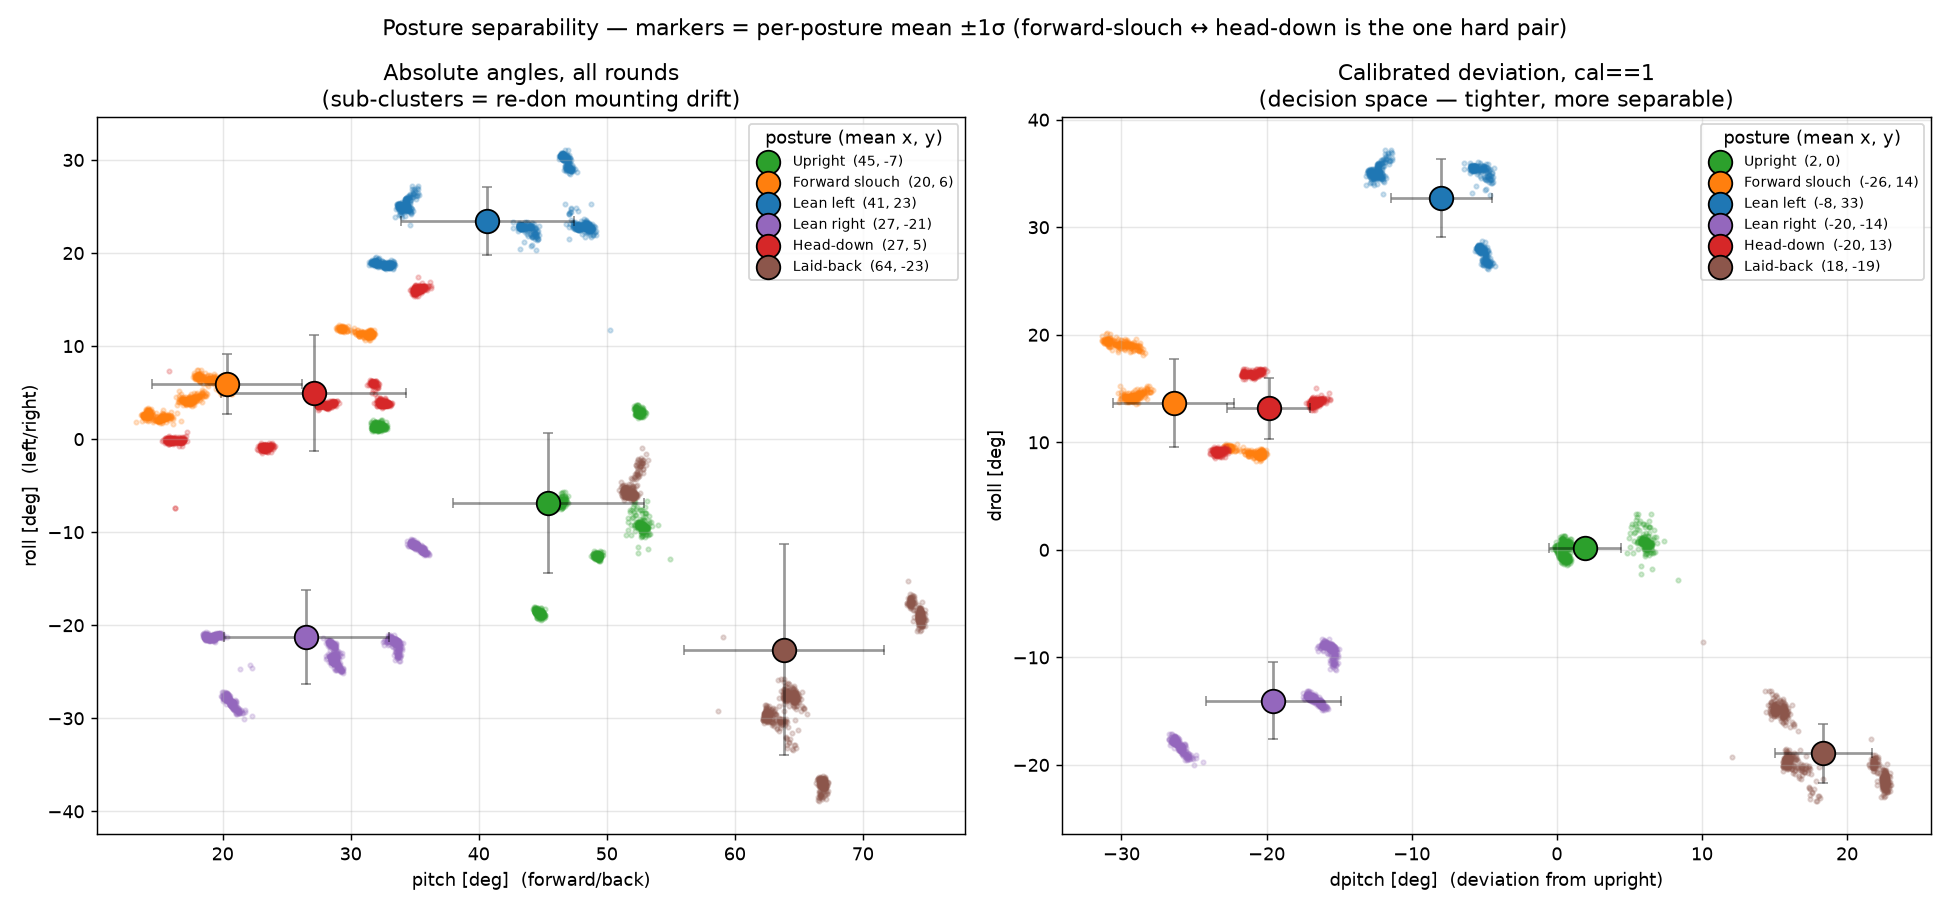
\includegraphics[width=0.9\linewidth]{02_separation.png}
  \fonte{\texttt{analysis/plot\_postures.py -\/-csv data/2026-06-19\_andre\_no-neck-mount\_own-chair.csv}}
\end{figure}

\paragraph{Deriva por remontagem (OE1).}
Recalculada a partir das retenções estáveis (\texttt{tag==0}), ao longo das
\textbf{4 épocas genuínas} de remontagem, a referência ``ereto'' desloca-se
$\sim$8{,}0\degree{} em pitch e $\sim$21{,}6\degree{} em roll
(Figura~\ref{fig:redon}). Ou seja, um \emph{limiar absoluto fixo} erraria após uma
remontagem, o que \textbf{justifica a calibração por usuário}. Esta é a evidência,
medida \emph{diretamente no dispositivo vestido}, por trás da decisão de projeto de
calibração documentada no repositório.

\begin{figure}[H]
  \centering
  \caption{Deriva da referência de ``ereto'' entre remontagens (re-don). A
  dispersão da referência ($\sim$8\degree{} pitch / $\sim$21{,}6\degree{} roll)
  fundamenta a calibração por usuário (OE1).}
  \label{fig:redon}
  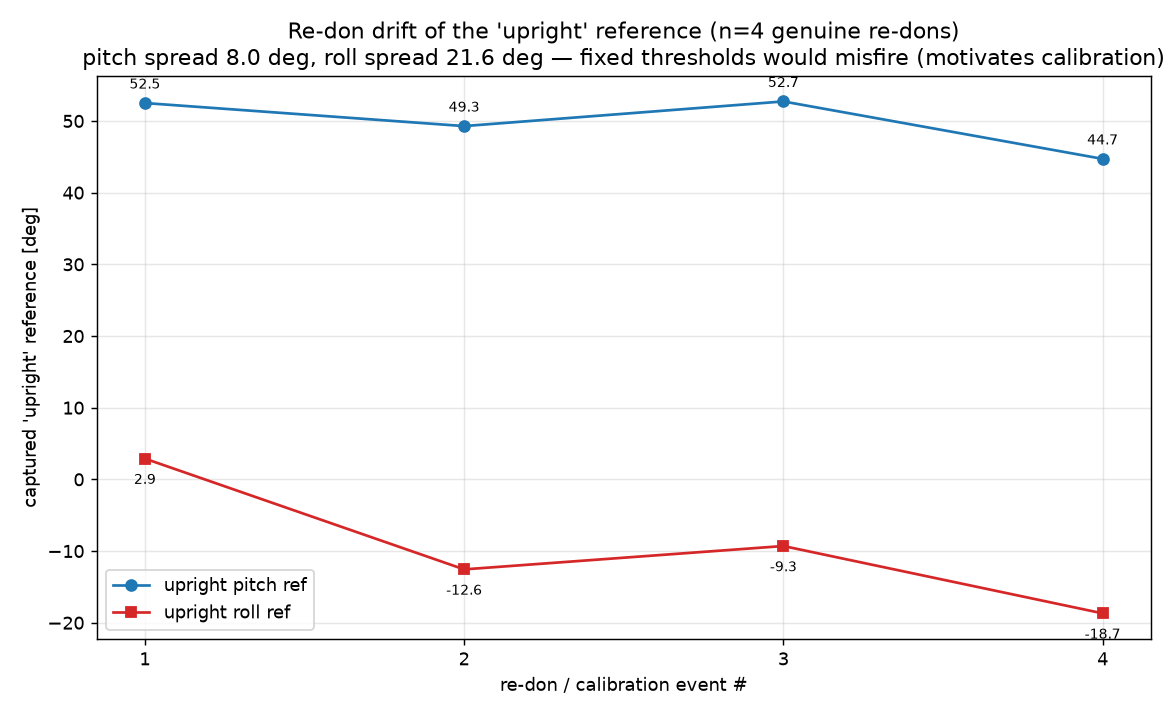
\includegraphics[width=0.85\linewidth]{04_redon_drift.png}
  \fonte{\texttt{analysis/plot\_postures.py -\/-csv data/2026-06-19\_andre\_no-neck-mount\_own-chair.csv}}
\end{figure}

\paragraph{Limiar de alerta proposto ($\approx$10\degree{}).}
Sentado ereto, o desvio $d$ fica $\leq 6{,}4\degree{}$ (p95); para as posturas ruins
mantidas, o p05 \emph{agregado} é $18{,}6\degree{}$ (a postura individual mais baixa
é $18{,}0\degree{}$, \texttt{tag~3}/inclinar à direita). Um limiar de
\textbf{10\degree{}} separa os dois regimes com \textbf{0\,\% de falsos alarmes e
100\,\% das posturas ruins capturadas} \emph{nesta base} (Figura~\ref{fig:alert}).
\textbf{Ressalva:} a margem é ampla porque as posturas foram executadas de forma
pronunciada; trata-se de um \emph{ponto de partida} a re-sintonizar em posturas
naturais e em mais sujeitos, não de uma figura de desempenho validada.

\begin{figure}[H]
  \centering
  \caption{Desvio em relação ao ereto calibrado por postura e o limiar de alerta
  proposto de $\sim$10\degree{}.}
  \label{fig:alert}
  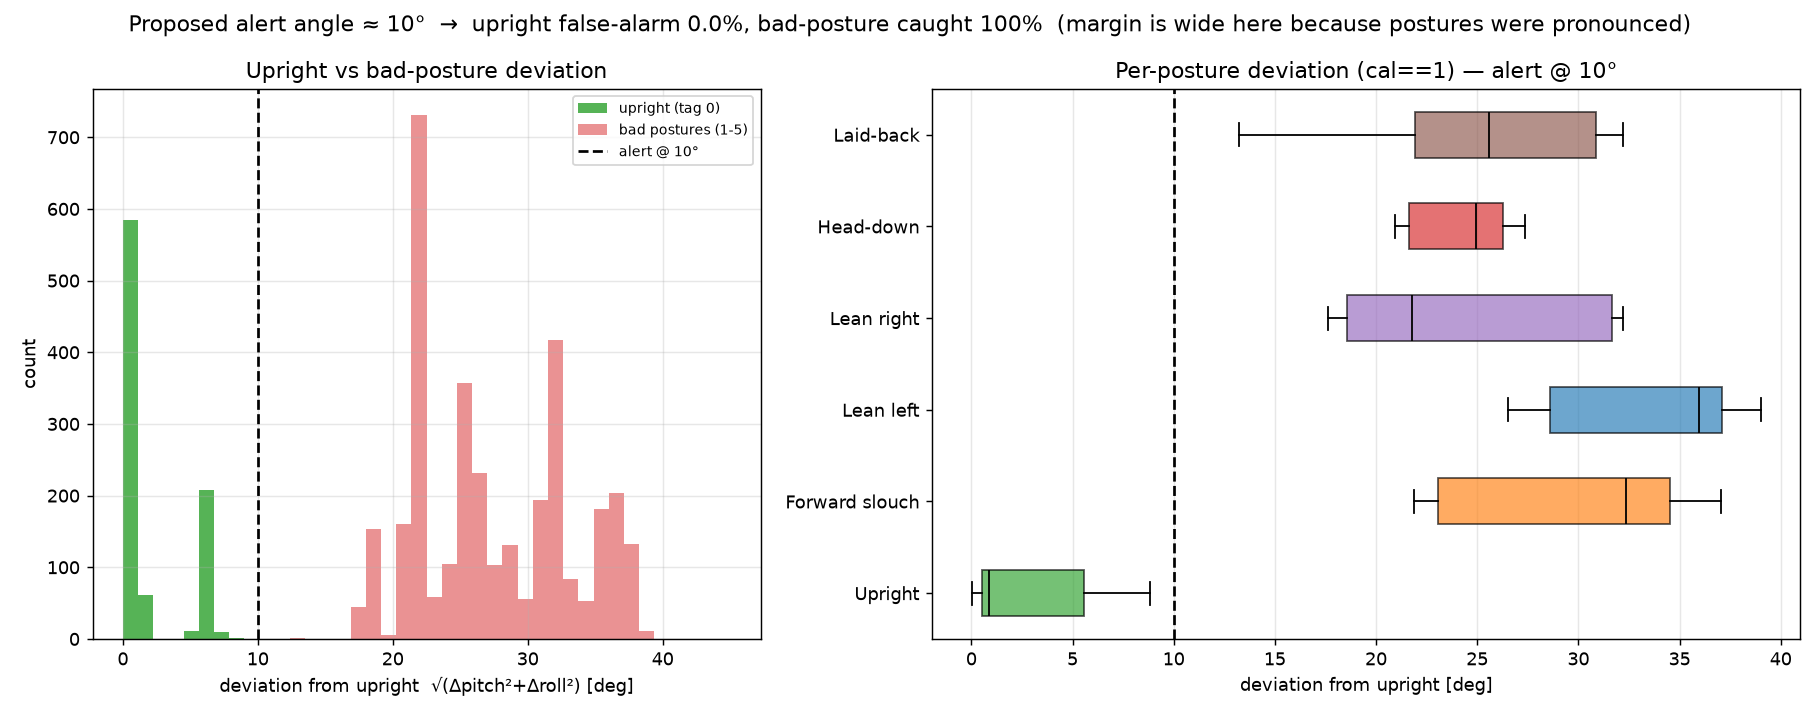
\includegraphics[width=0.85\linewidth]{06_alert_threshold.png}
  \fonte{\texttt{analysis/plot\_postures.py -\/-csv data/2026-06-19\_andre\_no-neck-mount\_own-chair.csv}}
\end{figure}

\noindent A saúde do sensor foi confirmada: $|g| = 0{,}993 \pm 0{,}004$\,g em
repouso, com toda excursão fora de faixa coincidindo com amostras de transição
(\texttt{tag==9}).

\subsection{Canal FSR (Campanha B)}

\paragraph{Curva resistência {\itshape vs.} carga e saturação.}
A resistência cai de $\sim$4134\,\ohm{} (toque leve) para $\sim$180\,\ohm{}, com o
\emph{joelho} de saturação por volta de $\sim$1{,}2\,kg (Figura~\ref{fig:curve}).
\textbf{Ressalva importante:} esse ``piso'' de 158--180\,\ohm{} é a resistência
\emph{no topo da escala (2\,kg)} --- um \textbf{limite superior} do piso real, não a
assíntota, pois um adulto sentado carrega muito além de 2\,kg. Portanto, a leitura
deve ser tratada como \textbf{pressão relativa / contato}, não força calibrada.

\begin{figure}[H]
  \centering
  \caption{R {\itshape vs.} carga (FSR1) com o joelho de saturação.}
  \label{fig:curve}
  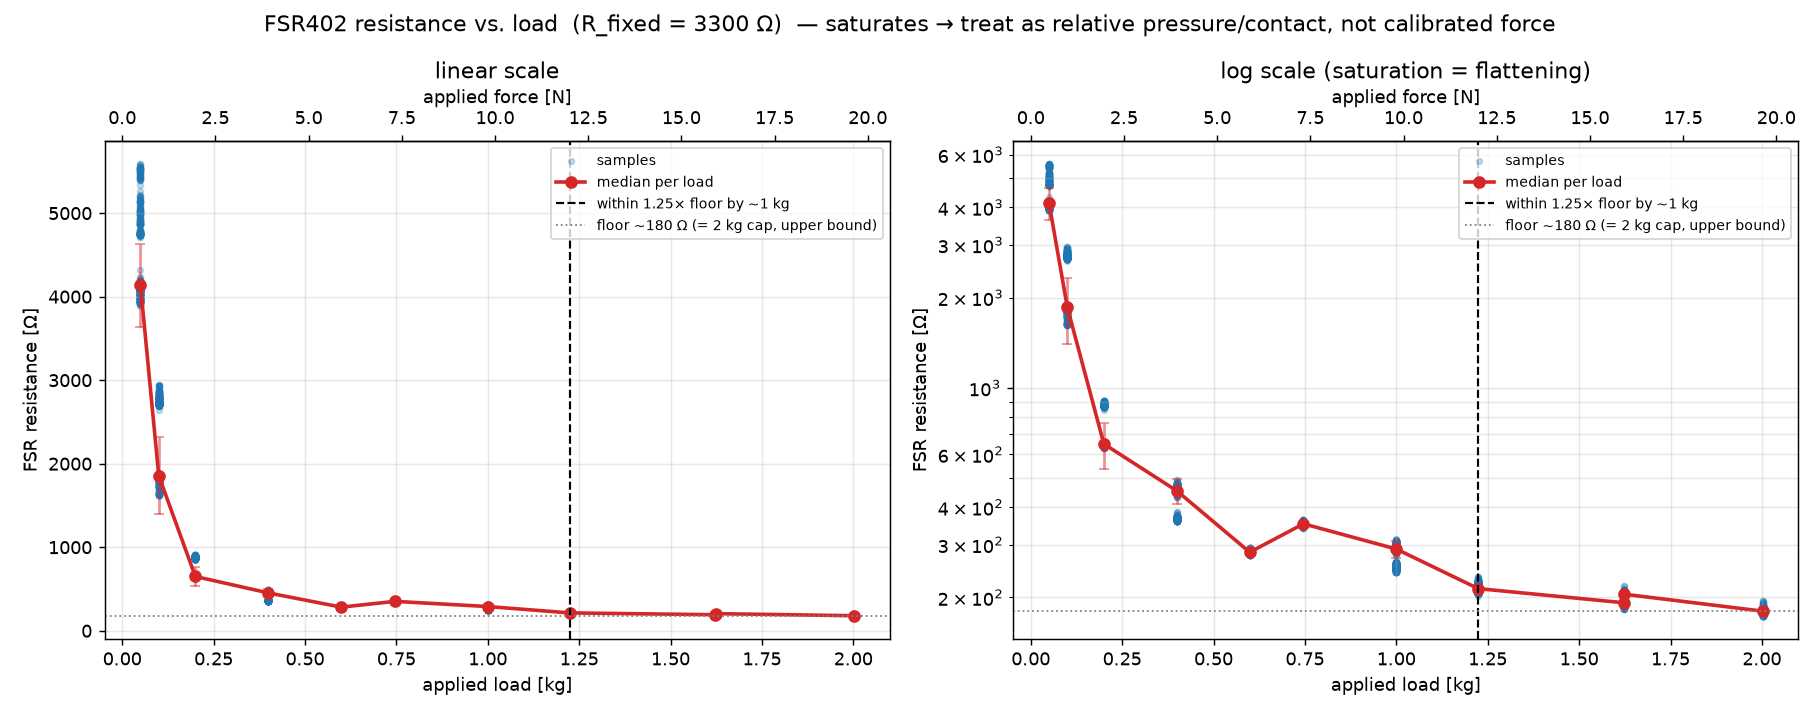
\includegraphics[width=0.85\linewidth]{fsr_curve.png}
  \fonte{\texttt{analysis/plot\_fsr\_curve.py -\/-units g}}
\end{figure}

\paragraph{Modelo de resposta e resolução.}
A resposta ajusta-se bem a uma lei de potência $R = a\,F^{b}$ ($R^2 \approx 0{,}97$),
mas a \textbf{condutância} $G = 1/R$ é aproximadamente \emph{linear} na força
($R^2 \approx 0{,}95$, contra $R^2 \approx 0{,}42$ para $R$ linear em $F$) ---
$G$ é a variável natural para um mapa de pressão relativa. A sensibilidade na faixa
operacional é de $\sim$10\,\ohm{}/100\,g; com o ADC de 10\,bits, isso dá
$\sim$3{,}1\,\ohm{}/contagem no piso ($\approx$1{,}7\,\% por contagem) ---
\textbf{poucas faixas de pressão resolvíveis} quando sentado (Figura~\ref{fig:model}).

\begin{figure}[H]
  \centering
  \caption{Ajuste lei de potência, linearidade da condutância e resolução do ADC.}
  \label{fig:model}
  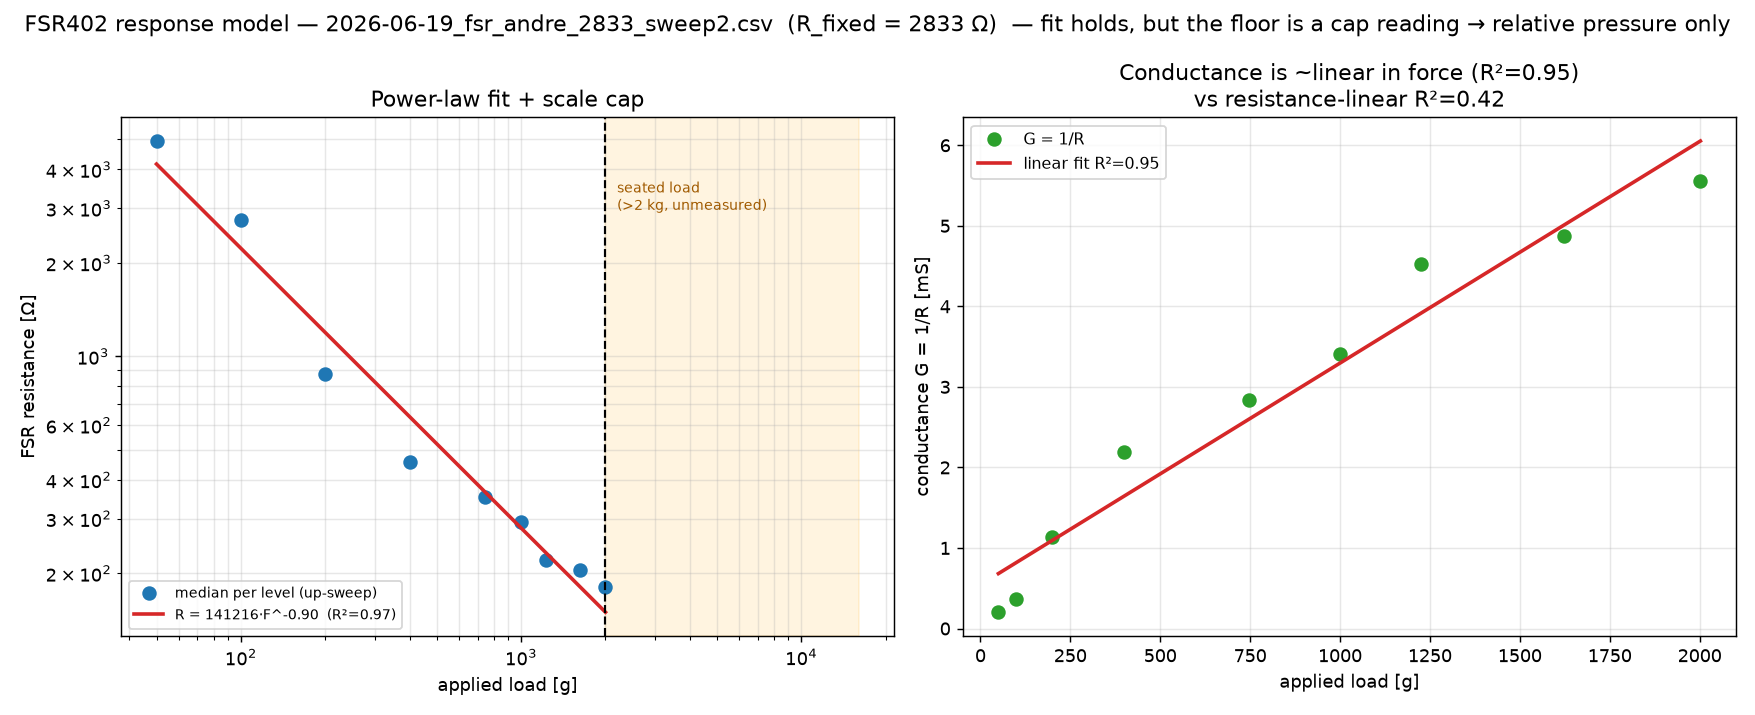
\includegraphics[width=0.9\linewidth]{fsr_model.png}
  \fonte{\texttt{analysis/plot\_fsr\_model.py}}
\end{figure}

\paragraph{Histerese.}
Comparando subida {\itshape vs.} descida (FSR2): a diferença vai de $-$76\,\%
em 50\,g a $-$6\,\% em 1\,kg; a histerese média absoluta é $\sim$52\,\% até 400\,g e
$\sim$6\,\% a partir de 1\,kg (Figura~\ref{fig:hyst}). \textbf{No regime operacional
(sentado), a resposta é praticamente independente da direção}; toda a bagunça vive no
toque leve.

\begin{figure}[H]
  \centering
  \caption{Laço de histerese (carga {\itshape vs.} descarga) por nível.}
  \label{fig:hyst}
  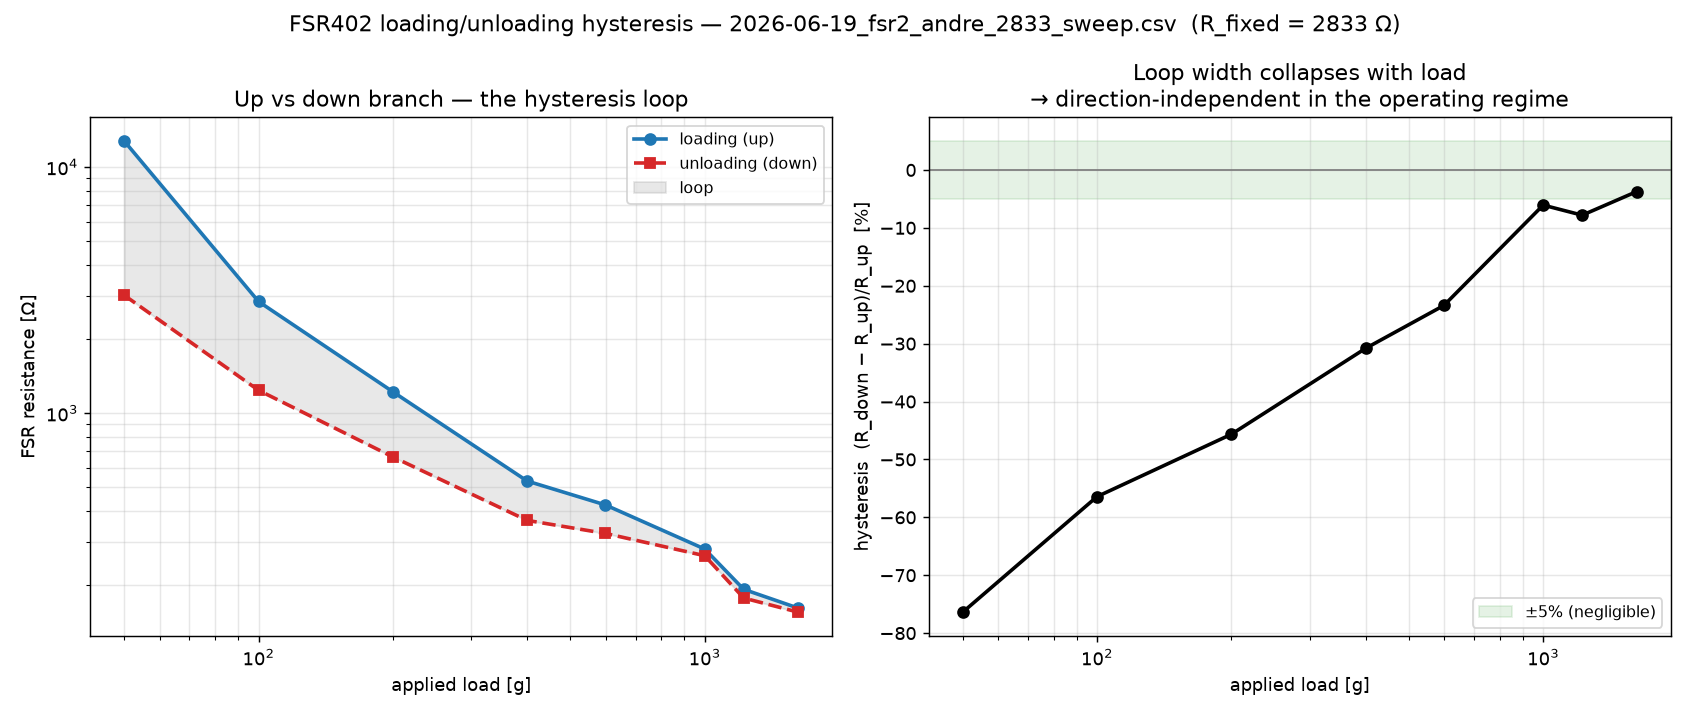
\includegraphics[width=0.85\linewidth]{fsr_hysteresis.png}
  \fonte{\texttt{analysis/plot\_fsr\_hysteresis.py}}
\end{figure}

\paragraph{Creep (deriva sob carga constante).}
Sob 1\,kg constante, a resistência deriva $-$7{,}4\,\% em 11\,min (FSR1) e
$-$11{,}5\,\% em 12\,min (FSR2) --- ou seja, a leitura ``afunda'' lentamente sob
carga sustentada (Figura~\ref{fig:creep}). Mais uma razão para tratar o FSR como
relativo, não calibrado, e para a recalibração periódica.

\begin{figure}[H]
  \centering
  \caption{Creep: resistência {\itshape vs.} tempo sob 1\,kg (FSR1, $-$7{,}4\,\% em
  11\,min).}
  \label{fig:creep}
  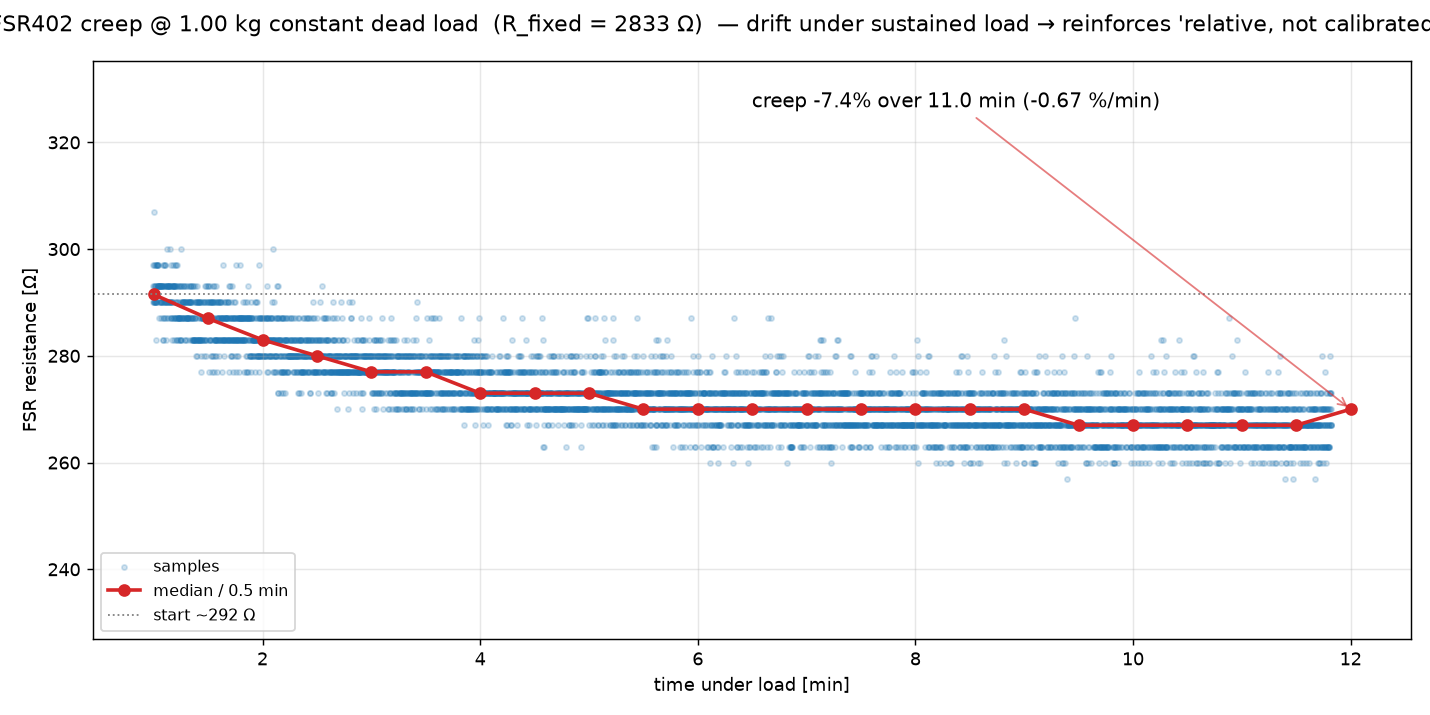
\includegraphics[width=0.85\linewidth]{fsr_creep.png}
  \fonte{\texttt{analysis/plot\_fsr\_creep.py -\/-units g}}
\end{figure}

\paragraph{Variação entre peças {\itshape vs.} montagem (o resultado forte).}
Usando uma \textbf{regra de direção única} (mediana de todas as amostras por nível),
a variação \emph{entre as 3 peças} é modesta no regime sentado e mais ruidosa em
cargas intermediárias (Tabela~\ref{tab:p2p}). Em contraste, a \textbf{variação por
assentamento/montagem} domina: o \emph{mesmo} sensor (FSR3) lê 3--11$\times$ mais
alto no toque leve enquanto o \emph{puck} ainda não assentou no pad (em 400\,g,
subida $\approx$9\,k\ohm{} contra descida 812\,\ohm{}), conforme os marcadores ocos
(\emph{seating-suspect}) na Figura~\ref{fig:p2p}.

\begin{table}[H]
  \centering
  \caption{Variação entre peças (medianas de todas as amostras por nível).
  Espalhamento $=(\max-\min)/\min$.}
  \label{tab:p2p}
  \begin{tabular}{rrrrr}
    \toprule
    Carga (g) & FSR1 (\ohm) & FSR2 (\ohm) & FSR3 (\ohm) & Espalhamento \\
    \midrule
    400   & 453 & 514 & 502 & 13\,\% \\
    1000  & 290 & 267 & 391 & 46\,\% \\
    1600  & 192 & 158 & 183 & 22\,\% \\
    2000  & 180 & 164 & 173 & 10\,\% \\
    \bottomrule
  \end{tabular}
  \fonte{\texttt{analysis/plot\_fsr\_parttopart.py -\/-both}}
\end{table}

\begin{figure}[H]
  \centering
  \caption{Sobreposição R {\itshape vs.} carga das 3 peças (esq.) e espalhamento
  {\itshape vs.} carga (dir.). Os transientes de assentamento (marcadores ocos
  $\triangledown$) excedem em muito a variação real entre peças.}
  \label{fig:p2p}
  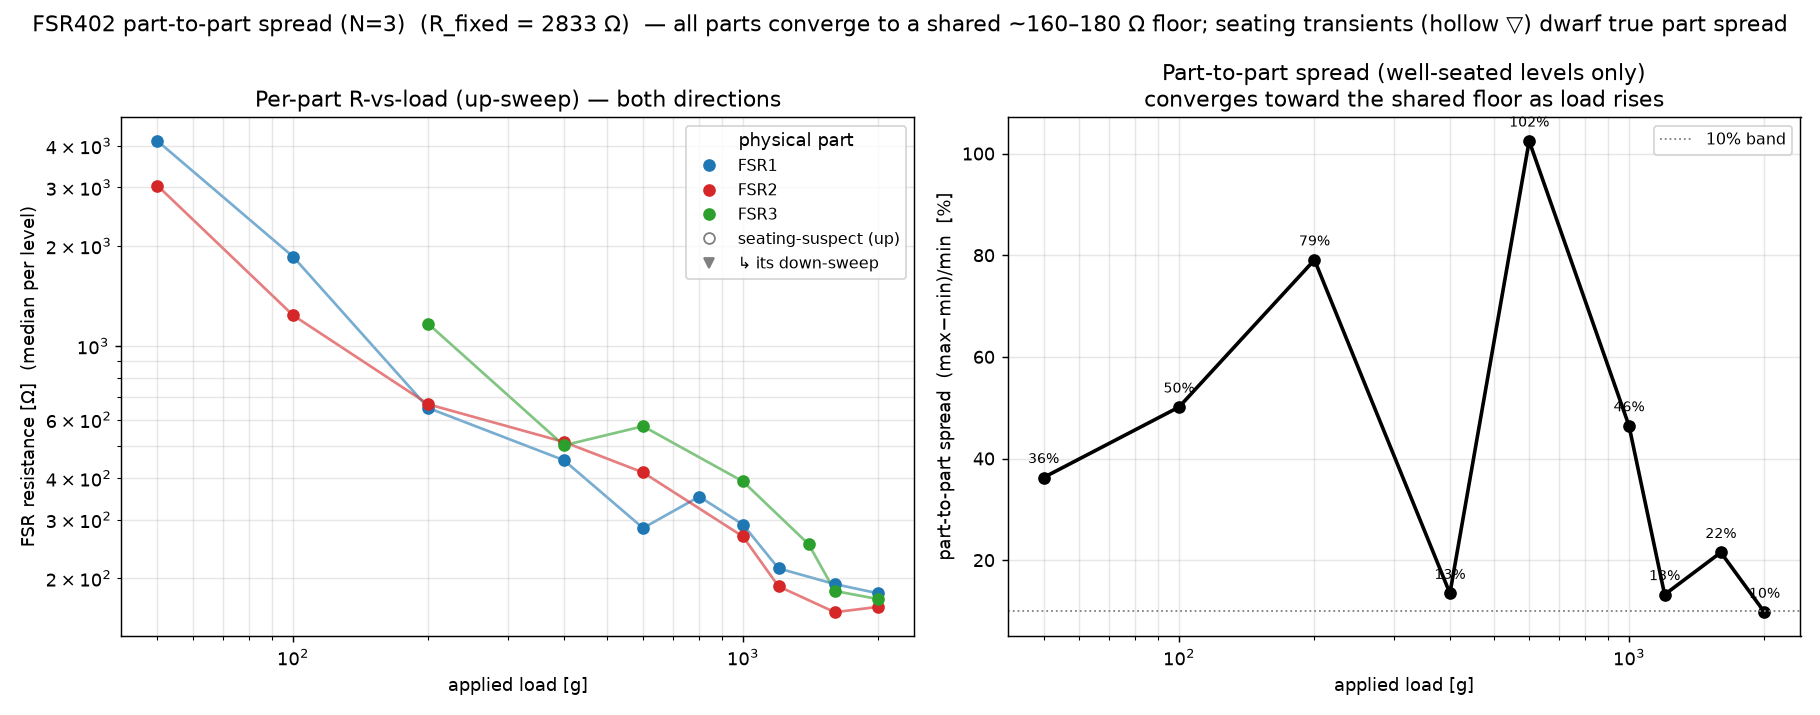
\includegraphics[width=\linewidth]{fsr_parttopart.png}
  \fonte{\texttt{analysis/plot\_fsr\_parttopart.py -\/-both}}
\end{figure}

\noindent\textbf{Leitura honesta deste resultado.} O fator 3--11$\times$ é um
\emph{transiente de bancada} (subida, \emph{puck} rígido não assentado): ele
demonstra a sensibilidade de montagem \emph{em princípio} e, somado à deriva por
remontagem do IMU, \textbf{motiva fortemente a calibração por instalação/usuário}.
A magnitude da variação no FSR \emph{de fato montado na espuma da cadeira, sob um
humano}, ainda não foi medida (Próximas etapas).

% =====================================================================
\section{Limitações e validade estatística}
\label{sec:limitacoes}
Esta é uma caracterização \textbf{descritiva de viabilidade}, e suas margens devem
ser lidas como tal:
\begin{itemize}[nosep]
  \item \textbf{Amostra:} 1 sujeito (IMU) e 3 sensores (FSR), em sessão única, num
        único dia. Nenhuma estatística inferencial (intervalos de confiança /
        significância) é reivindicada --- nem seria justificada neste $N$.
  \item \textbf{Posturas pronunciadas:} as posturas do IMU foram executadas de forma
        deliberadamente exagerada, de modo que as margens de separação (par
        1{$\leftrightarrow$}4 e limiar de 10\degree{}) são \textbf{limites
        superiores otimistas}; a separação realista é uma questão em aberto.
  \item \textbf{Bancada $\neq$ cadeira:} os FSR foram medidos sob um \emph{puck}
        rígido sobre balança, não na cadeira instrumentada com espuma. O fator de
        assentamento 3--11$\times$ é um transiente de bancada.
  \item \textbf{Sem fusão:} os canais foram caracterizados isoladamente; não há
        captura conjunta FSR\,+\,IMU.
  \item \textbf{Ambiente não controlado:} temperatura e horário não foram fixados; o
        FSR402 deriva com ambos.
  \item \textbf{Limites do canal FSR:} o ``piso'' de resistência é um limite superior
        (topo da escala de 2\,kg); a resolução sentada é grosseira
        ($\sim$1{,}7\,\%/contagem) --- adequada a \emph{contato/pressão relativa},
        não a força calibrada.
\end{itemize}

% =====================================================================
\section{Próximas etapas}
\label{sec:proximas}
\begin{itemize}[nosep]
  \item \textbf{Mapa de pressão de 6 canais do assento} (\texttt{uno\_fsr6\_test},
        A0--A5): o contraste esquerda/direita e frente/trás é a própria premissa do
        canal-cadeira --- entregável ainda não capturado nesta parcial.
  \item \textbf{Fusão FSR\,+\,IMU:} a novidade do trabalho frente ao BackWatch;
        primeira captura conjunta/contemporânea.
  \item \textbf{Integração de hardware:} segundo XIAO nRF52840 + rádio ESB
        (link cadeira{$\leftrightarrow$}corpo), multiplexador CD74HC4067 (10 FSR),
        bateria 1S LiPo, enclosure vestível e cadeira instrumentada com a
        disposição final dos sensores.
  \item \textbf{Comunicação com o usuário (OE3):} acionamento do motor de vibração
        e a lógica de alerta no dispositivo.
  \item \textbf{Repetições para a margem realista:} \emph{neck mount}, posturas
        naturais (não pronunciadas) e múltiplos sujeitos.
  \item \textbf{Piso real do FSR:} $R_{\text{fixo}}$ menor ($\sim$1\,k\ohm) e escala
        maior, para alcançar a saturação real além de 2\,kg.
  \item \textbf{Avaliação de eficiência (OE4):} possível apenas após a montagem do
        sistema fundido.
\end{itemize}

% =====================================================================
\section*{Referências}
\addcontentsline{toc}{section}{Referências}
% NOTA: referências completadas/conferidas nesta versão (Iida & Guimarães, Dul,
% Grandjean, Kuorinka, McAtamney/Corlett, Sonne/Villalta/Andrews [ROSA], Okezue,
% Mohammadian, Robertson). PENDENTE: FERREIRA et al. (BackWatch, 2023), cujos dados
% bibliográficos ainda precisam ser confirmados [completar].
\begin{description}[leftmargin=1.5em,style=nextline,nosep]
  \item[DUL, J.; WEERDMEESTER, B.] \emph{Ergonomia prática}. 3. ed. São Paulo:
        Edgard Blücher, 2012.
  \item[FERREIRA et al.] \emph{BackWatch}: sistema de monitoramento de inclinação de
        tronco e cabeça, 2023. [completar dados bibliográficos]
  \item[GRANDJEAN, E.] \emph{Manual de ergonomia: adaptando o trabalho ao homem}.
        4. ed. Porto Alegre: Bookman, 1998.
  \item[IIDA, I.; GUIMARÃES, L. B. M.] \emph{Ergonomia: projeto e produção}. 3. ed.
        São Paulo: Edgard Blücher, 2016.
  \item[KUORINKA, I. et al.] Standardised Nordic questionnaires for the analysis of
        musculoskeletal symptoms. \emph{Applied Ergonomics}, v. 18, n. 3,
        p. 233--237, 1987.
  \item[McATAMNEY, L.; CORLETT, E. N.] RULA: a survey method for the investigation of
        work-related upper limb disorders. \emph{Applied Ergonomics}, v. 24, n. 2,
        p. 91--99, 1993.
  \item[MOHAMMADIAN et al.] Musculoskeletal disorders among office workers:
        prevalence, ergonomic risk factors, and their interrelationships.
        \emph{Scientific Reports}, v. 15, 2025. DOI: 10.1038/s41598-025-30155-6.
  \item[OKEZUE, O. C. et al.] Work-Related Musculoskeletal Disorders among Office
        Workers in Higher Education Institutions: A Cross-Sectional Study.
        \emph{Ethiopian Journal of Health Sciences}, v. 30, n. 5, p. 715--724, 2020.
  \item[ROBERTSON, M.; CIRIELLO, V.; GARABET, A.] Office ergonomics training and a
        sit-stand workstation: effects on musculoskeletal and visual symptoms and
        performance of office workers. \emph{Applied Ergonomics}, v. 44, n. 1,
        p. 73--85, 2013.
  \item[SONNE, M.; VILLALTA, D. L.; ANDREWS, D. M.] Development and evaluation of an
        office ergonomic risk checklist: ROSA --- Rapid Office Strain Assessment.
        \emph{Applied Ergonomics}, v. 43, n. 1, p. 98--108, 2012.
\end{description}

\end{document}
